% !TEX program = lualatex
\documentclass[a4paper,10pt,oneside,openany]{ltjsreport}
\usepackage[margin=21mm,top=19mm,bottom=20mm]{geometry}
\usepackage[haranoaji]{luatexja-preset}
\usepackage{amsmath,amssymb,graphicx,booktabs,longtable,xcolor,float}
\usepackage[unicode,colorlinks=true,linkcolor=blue!45!black,urlcolor=blue!45!black]{hyperref}
\usepackage{caption}
\captionsetup{font=small,labelfont=bf}
\setcounter{tocdepth}{0}
\setlength{\parskip}{0.45em}
\setlength{\parindent}{1em}
\raggedbottom
\newcommand{\sourcefile}[1]{{\small\texttt{\detokenize{#1}}}}
\begin{document}


\title{\Huge 実験4\\[0.6em]\LARGE スピン偏極依存性\\[1em]\large 一次元HubbardモデルのUHF計算}

\author{保存結果の解析レポート}\date{2026年11月2日}\maketitle

\chapter*{概要}

半充填を保って $\Delta N=0,2,4,12$ と増やす。OBCは全条件で収束し、PBCは $\Delta N=2$ のみ未収束となった。OBCのエネルギーは偏極とともに上昇するが、局所磁化の平均絶対値はわずかに増大する。磁化の振幅と交互配列の整合性は別の量である。

対象は8ケース、保存図33枚である。収束は7ケース、未収束は1ケース。本書では生成物の種類ごとに章を設け、同じ条件のOBCとPBCを並べて読む。

\tableofcontents

\chapter{計算ログ：条件と最終結果}

\sourcefile{uhf_results.txt}

\section*{計算条件と量の定義}

$L=50$、$t=1$、温度 $T=0$、外部電場なし。全エネルギーと軌道エネルギーは $t$ を単位とする。
OBCは開放端、PBCはサイト50と1も接続する周期境界である。$N_e=N_\uparrow+N_\downarrow$、$\Delta N=N_\uparrow-N_\downarrow$ と定義する。
収束判定は混合前の密度残差 $r<10^{-10}$、最大反復回数は10000である。
表の「未」は未収束の最終再評価値であり、その桁数は精度保証ではない。

\begin{center}\small\setlength{\tabcolsep}{4pt}
\begin{longtable}{lrrrr}
\toprule
条件 & $N_e$ & $\Delta N$ & $U/t$ & mixing \\ \midrule
\endhead
dN00 & 50 & 0 & 4 & 0.25 \\
dN02 & 50 & 2 & 4 & 0.25 \\
dN04 & 50 & 4 & 4 & 0.25 \\
dN12 & 50 & 12 & 4 & 0.25 \\
\bottomrule\end{longtable}\end{center}

\section*{最終エネルギー}

$E=E_{\rm kin}+E_{\rm int}$、$E_{\rm int}=U\sum_i n_{i\uparrow}n_{i\downarrow}$。全エネルギーは占有軌道固有値の単純な総和ではなく、平均場の二重計数を除いた量である。

\begin{center}\small\setlength{\tabcolsep}{4pt}
\begin{longtable}{lrrrr}
\toprule
条件/境界 & 状態 & $E$ & $E_{\rm kin}$ & $E_{\rm int}$ \\ \midrule
\endhead
dN00/OBC & 収束 & -23.013070704 & -43.110712440 & 20.097641737 \\
dN00/PBC & 収束 & -23.455261995 & -43.889991764 & 20.434729770 \\
dN02/OBC & 収束 & -22.174831178 & -41.775151618 & 19.600320440 \\
dN02/PBC & 未 & -20.391716039 & -43.552607432 & 23.160891393 \\
dN04/OBC & 収束 & -21.794883924 & -41.243290301 & 19.448406377 \\
dN04/PBC & 収束 & -21.778774482 & -41.218743972 & 19.439969490 \\
dN12/OBC & 収束 & -18.758709657 & -37.015897060 & 18.257187403 \\
dN12/PBC & 収束 & -18.742650577 & -36.991979749 & 18.249329172 \\
\bottomrule\end{longtable}\end{center}

半充填を保って $\Delta N=0,2,4,12$ と増やす。OBCは全条件で収束し、PBCは $\Delta N=2$ のみ未収束となった。OBCのエネルギーは偏極とともに上昇するが、局所磁化の平均絶対値はわずかに増大する。磁化の振幅と交互配列の整合性は別の量である。

\section*{原資料と再利用}

出典は \sourcefile{results_vault/experiment_04/} 内の各条件/OBC・PBCのログ、CSV、PNG。\\ 補助資料は \sourcefile{experiment_conditions.md} と \sourcefile{uhf.jl}。値は保存済みの結果から採り、SCFを再実行していない。

条件名は原資料のディレクトリ名である。dN00は実験2の再利用。

再利用データは独立した追加試行ではない。本書の解釈は保存された有限サイズ・UHF解の範囲に限る。

\chapter{密度CSV：電荷分布と二重占有}

\sourcefile{density_checkpoint.csv}

CSVの50サイトすべてから $q_i=n_{i\uparrow}+n_{i\downarrow}$、$m_i=n_{i\uparrow}-n_{i\downarrow}$、
$D=L^{-1}\sum_i n_{i\uparrow}n_{i\downarrow}$ を計算した。密度の各スピン成分は0以上1以下で、総和は指定した粒子数に一致することを確認した。未収束時のCSVは最後の混合密度を対角化して得た出力密度であり、固定点の密度とは限らない。

\begin{center}\small\setlength{\tabcolsep}{4pt}
\begin{longtable}{lrrrr}
\toprule
条件/境界 & 状態 & $\min q_i$ & $\max q_i$ & $D$ \\ \midrule
\endhead
dN00/OBC & 収束 & 1.000000 & 1.000000 & 0.100488 \\
dN00/PBC & 収束 & 1.000000 & 1.000000 & 0.102174 \\
dN02/OBC & 収束 & 1.000000 & 1.000000 & 0.098002 \\
dN02/PBC & 未 & 0.318809 & 1.681191 & 0.115804 \\
dN04/OBC & 収束 & 1.000000 & 1.000000 & 0.097242 \\
dN04/PBC & 収束 & 1.000000 & 1.000000 & 0.097200 \\
dN12/OBC & 収束 & 1.000000 & 1.000000 & 0.091286 \\
dN12/PBC & 収束 & 1.000000 & 1.000000 & 0.091247 \\
\bottomrule\end{longtable}\end{center}

収束ケースでは電荷密度は一様な $q_i=1$ である。平均磁化は粒子数制約により $\Delta N/50=0,0.04,0.08,0.24$ と決まる。未収束の $\Delta N=2$・PBCでは電荷密度が約0.3188--1.6812と大きく変動しており、この分布を平衡状態の電荷秩序と解釈すべきではない。

\chapter{SCFエネルギー：反復による変化}

\sourcefile{scf_energy.png}

OBCでは $\Delta N=0$ から12で運動エネルギーが約6.094815増加し、相互作用エネルギーは約1.840454低下する。その結果、全エネルギーは約4.254361上昇する。偏極による二重占有の抑制は相互作用項を下げるが、運動項の増加を補えない。PBCの12では長い平坦区間の後にエネルギーが大きく低下しており、途中の停滞を最終状態と見誤らないことが重要である。

各図の横軸は反復回数、縦軸は各反復で評価した全エネルギーである。図ごとに軸範囲が異なるため、見かけの傾きだけを比較しない。最終ログ値は反復終了後の再評価であり、履歴の最終点とわずかに異なる場合がある。

\begin{center}\small\setlength{\tabcolsep}{4pt}
\begin{longtable}{lrrr}
\toprule
条件/境界 & 初回 $E$ & 最終 $E$ & 最後の履歴の $|\Delta E|$ \\ \midrule
\endhead
dN00/OBC & -17.140038 & -23.013071 & $0$ \\
dN00/PBC & -17.699645 & -23.455262 & $0$ \\
dN02/OBC & -15.794350 & -22.174831 & $0$ \\
dN02/PBC & -16.254906 & -20.391716 & $0$ \\
dN04/OBC & -14.724983 & -21.794884 & $0$ \\
dN04/PBC & -15.268191 & -21.778774 & $0$ \\
dN12/OBC & -11.720148 & -18.758710 & $0$ \\
dN12/PBC & -12.164555 & -18.742651 & $0$ \\
\bottomrule\end{longtable}\end{center}

\begin{figure}[H]\centering

\begin{minipage}{0.49\linewidth}\centering

\textbf{OBC：収束}\par

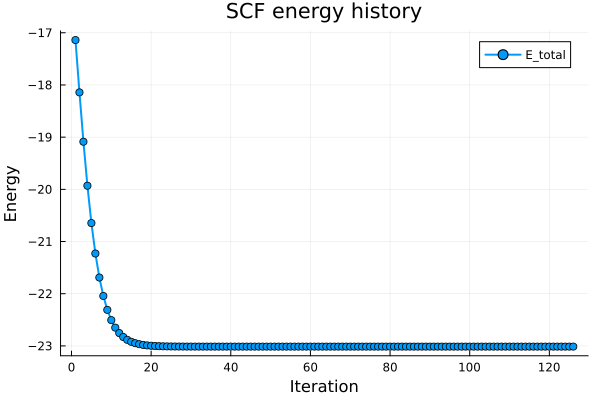
\includegraphics[width=\linewidth]{../../results_vault/experiment_04/dN00/OBC/scf_energy.png}

\end{minipage}\hfill%
\begin{minipage}{0.49\linewidth}\centering

\textbf{PBC：収束}\par

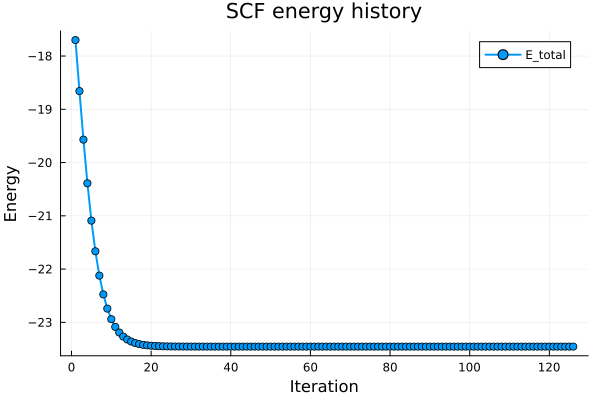
\includegraphics[width=\linewidth]{../../results_vault/experiment_04/dN00/PBC/scf_energy.png}

\end{minipage}

\caption{dN00。SCFエネルギーの比較。左：OBC、右：PBC。}\end{figure}

\begin{figure}[H]\centering

\begin{minipage}{0.49\linewidth}\centering

\textbf{OBC：収束}\par

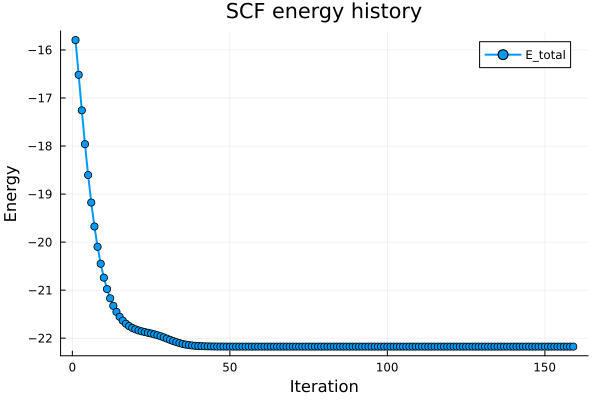
\includegraphics[width=\linewidth]{../../results_vault/experiment_04/dN02/OBC/scf_energy.png}

\end{minipage}\hfill%
\begin{minipage}{0.49\linewidth}\centering

\textbf{PBC：未収束・暫定}\par

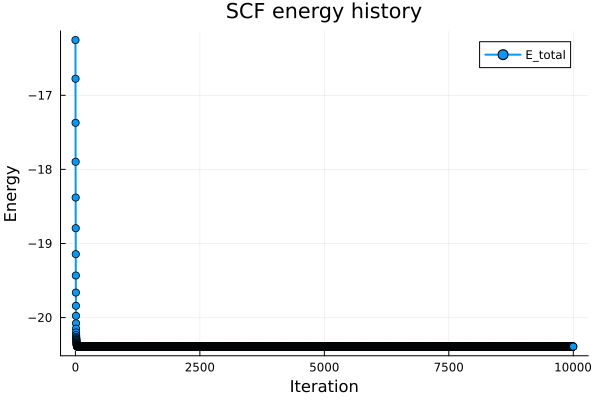
\includegraphics[width=\linewidth]{../../results_vault/experiment_04/dN02/PBC/scf_energy.png}

\end{minipage}

\caption{dN02。SCFエネルギーの比較。左：OBC、右：PBC。}\end{figure}

\begin{figure}[H]\centering

\begin{minipage}{0.49\linewidth}\centering

\textbf{OBC：収束}\par

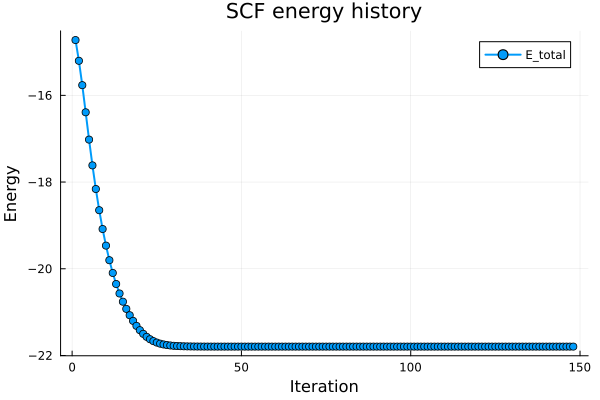
\includegraphics[width=\linewidth]{../../results_vault/experiment_04/dN04/OBC/scf_energy.png}

\end{minipage}\hfill%
\begin{minipage}{0.49\linewidth}\centering

\textbf{PBC：収束}\par

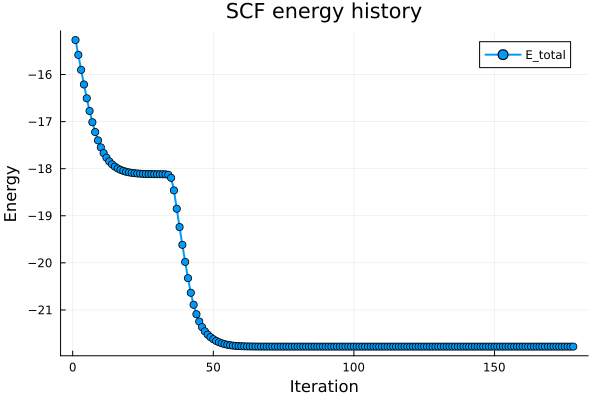
\includegraphics[width=\linewidth]{../../results_vault/experiment_04/dN04/PBC/scf_energy.png}

\end{minipage}

\caption{dN04。SCFエネルギーの比較。左：OBC、右：PBC。}\end{figure}

\begin{figure}[H]\centering

\begin{minipage}{0.49\linewidth}\centering

\textbf{OBC：収束}\par

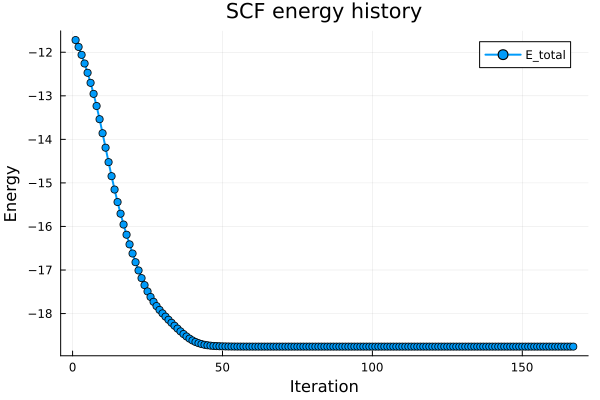
\includegraphics[width=\linewidth]{../../results_vault/experiment_04/dN12/OBC/scf_energy.png}

\end{minipage}\hfill%
\begin{minipage}{0.49\linewidth}\centering

\textbf{PBC：収束}\par

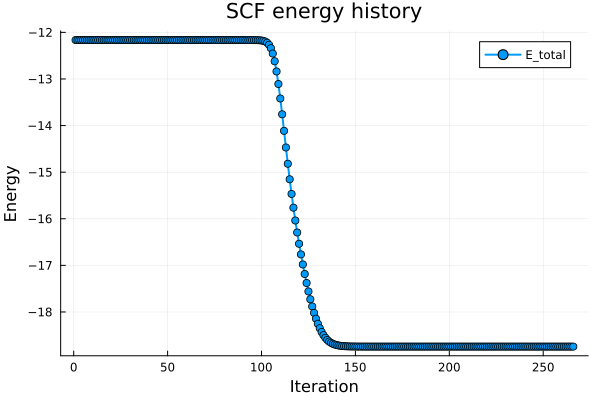
\includegraphics[width=\linewidth]{../../results_vault/experiment_04/dN12/PBC/scf_energy.png}

\end{minipage}

\caption{dN12。SCFエネルギーの比較。左：OBC、右：PBC。}\end{figure}

\chapter{SCF残差：自己無撞着性}

\sourcefile{scf_residual.png}

$\Delta N=2$・PBCの最終残差は0.3893であり、丸め誤差程度の未収束ではない。4および12のPBCでは途中で残差が再増加した後に収束し、それぞれ178、266反復を要する。OBCの148、167反復と比べ、同じ偏極でもPBCの密度再配列に長い過程がある。

残差は $r=\max_{i,\sigma}|F[n]_{i\sigma}-n_{i\sigma}|$。表は最終再評価値である。収束時には出力密度を採用してから再評価するため、履歴図の最後の残差とは同じとは限らない。

\begin{center}\small\setlength{\tabcolsep}{4pt}
\begin{longtable}{lrrr}
\toprule
条件/境界 & 状態 & 反復数 & 最終残差 \\ \midrule
\endhead
dN00/OBC & 収束 & 126 & $3.266\times10^{-11}$ \\
dN00/PBC & 収束 & 126 & $3.263\times10^{-11}$ \\
dN02/OBC & 収束 & 159 & $3.697\times10^{-11}$ \\
dN02/PBC & 未 & 10000 & $3.893\times10^{-1}$ \\
dN04/OBC & 収束 & 148 & $3.455\times10^{-11}$ \\
dN04/PBC & 収束 & 178 & $3.295\times10^{-11}$ \\
dN12/OBC & 収束 & 167 & $3.699\times10^{-11}$ \\
dN12/PBC & 収束 & 266 & $3.591\times10^{-11}$ \\
\bottomrule\end{longtable}\end{center}

\begin{figure}[H]\centering

\begin{minipage}{0.49\linewidth}\centering

\textbf{OBC：収束}\par

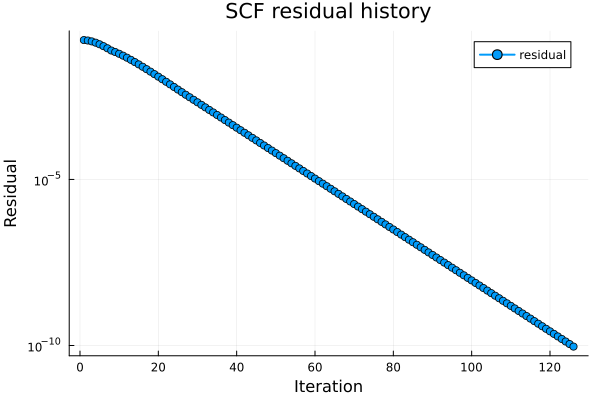
\includegraphics[width=\linewidth]{../../results_vault/experiment_04/dN00/OBC/scf_residual.png}

\end{minipage}\hfill%
\begin{minipage}{0.49\linewidth}\centering

\textbf{PBC：収束}\par

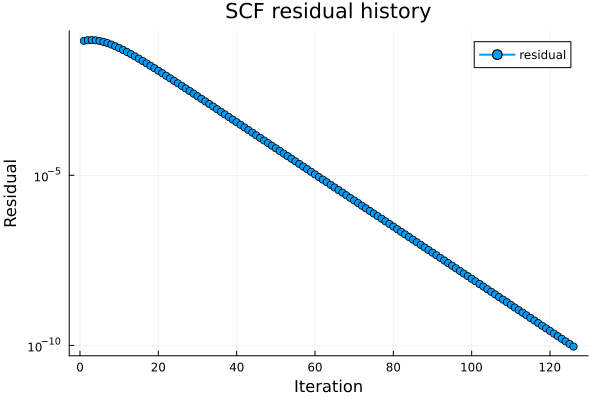
\includegraphics[width=\linewidth]{../../results_vault/experiment_04/dN00/PBC/scf_residual.png}

\end{minipage}

\caption{dN00。SCF残差の比較。左：OBC、右：PBC。}\end{figure}

\begin{figure}[H]\centering

\begin{minipage}{0.49\linewidth}\centering

\textbf{OBC：収束}\par

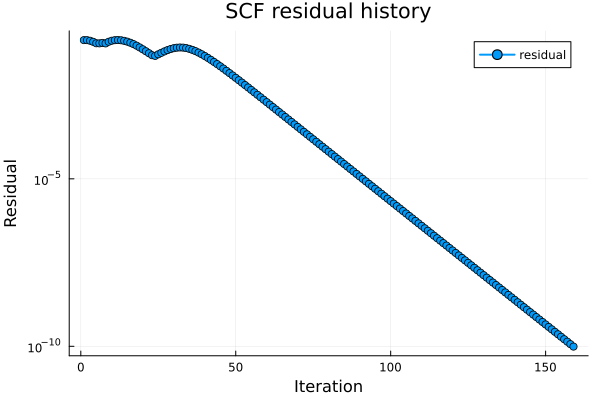
\includegraphics[width=\linewidth]{../../results_vault/experiment_04/dN02/OBC/scf_residual.png}

\end{minipage}\hfill%
\begin{minipage}{0.49\linewidth}\centering

\textbf{PBC：未収束・暫定}\par

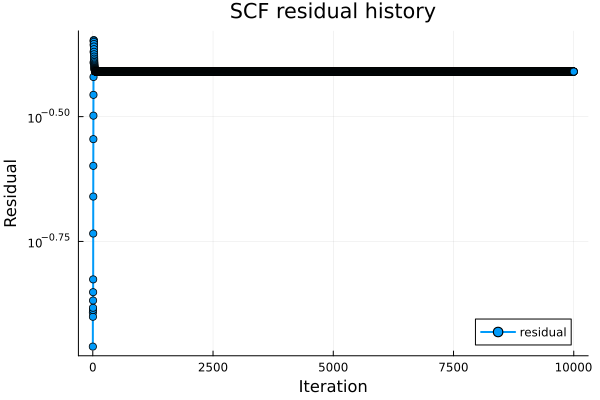
\includegraphics[width=\linewidth]{../../results_vault/experiment_04/dN02/PBC/scf_residual.png}

\end{minipage}

\caption{dN02。SCF残差の比較。左：OBC、右：PBC。}\end{figure}

\begin{figure}[H]\centering

\begin{minipage}{0.49\linewidth}\centering

\textbf{OBC：収束}\par

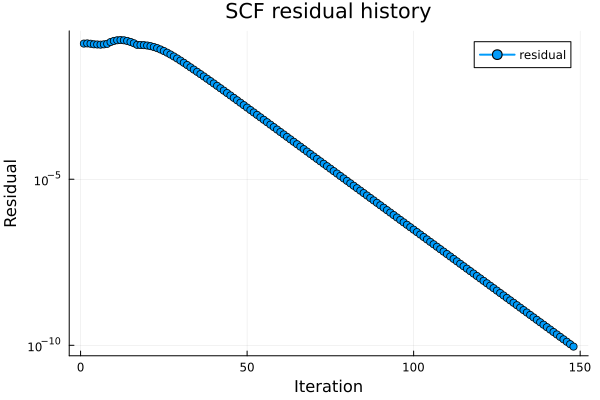
\includegraphics[width=\linewidth]{../../results_vault/experiment_04/dN04/OBC/scf_residual.png}

\end{minipage}\hfill%
\begin{minipage}{0.49\linewidth}\centering

\textbf{PBC：収束}\par

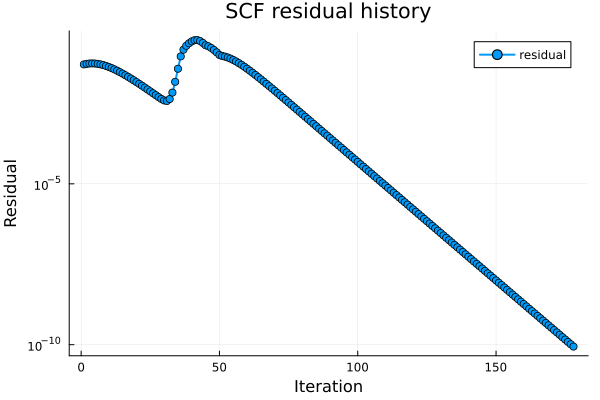
\includegraphics[width=\linewidth]{../../results_vault/experiment_04/dN04/PBC/scf_residual.png}

\end{minipage}

\caption{dN04。SCF残差の比較。左：OBC、右：PBC。}\end{figure}

\begin{figure}[H]\centering

\begin{minipage}{0.49\linewidth}\centering

\textbf{OBC：収束}\par

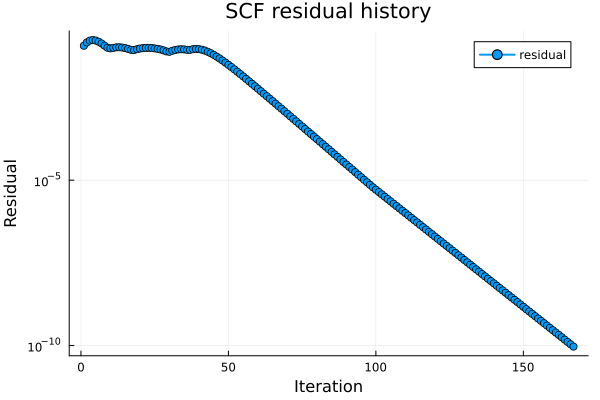
\includegraphics[width=\linewidth]{../../results_vault/experiment_04/dN12/OBC/scf_residual.png}

\end{minipage}\hfill%
\begin{minipage}{0.49\linewidth}\centering

\textbf{PBC：収束}\par

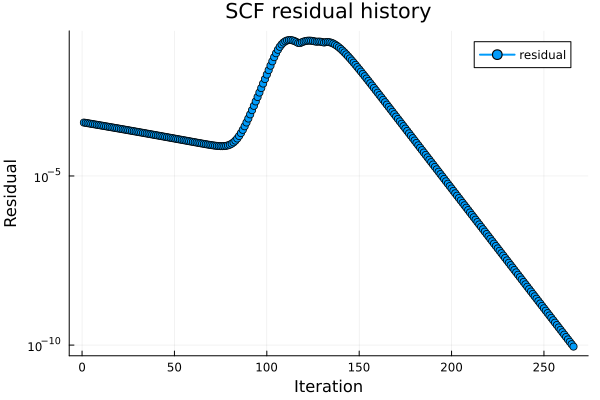
\includegraphics[width=\linewidth]{../../results_vault/experiment_04/dN12/PBC/scf_residual.png}

\end{minipage}

\caption{dN12。SCF残差の比較。左：OBC、右：PBC。}\end{figure}

\chapter{軌道エネルギー：準位構造}

\sourcefile{final_orbital_energies.png}

非偏極では上下スピンの準位が重なるが、偏極を増すと中央付近や端の準位で分離が現れる。占有準位数は上下で異なるため、常に25番目と26番目だけを比較するのは不適切であり、$N_\uparrow$ と $N_\downarrow$ に対応する占有境界を考える必要がある。図のスピン分裂は一様な剛体シフトだけでは説明できない。

横軸はエネルギー昇順の軌道番号、縦軸は $h_\sigma=h_0+U\operatorname{diag}(n_{\bar\sigma})$ の固有値である。固有値の数値ファイルは保存されていないため、図からの解釈は定性的なものに留める。未収束例をCSVから再対角化すると保存図とは異なる平均場になる可能性があり、本書ではその置換を行わない。

\begin{figure}[H]\centering

\begin{minipage}{0.49\linewidth}\centering

\textbf{OBC：収束}\par

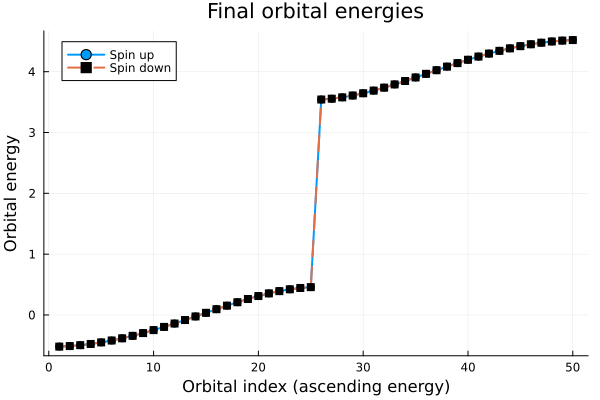
\includegraphics[width=\linewidth]{../../results_vault/experiment_04/dN00/OBC/final_orbital_energies.png}

\end{minipage}\hfill%
\begin{minipage}{0.49\linewidth}\centering

\textbf{PBC：収束}\par

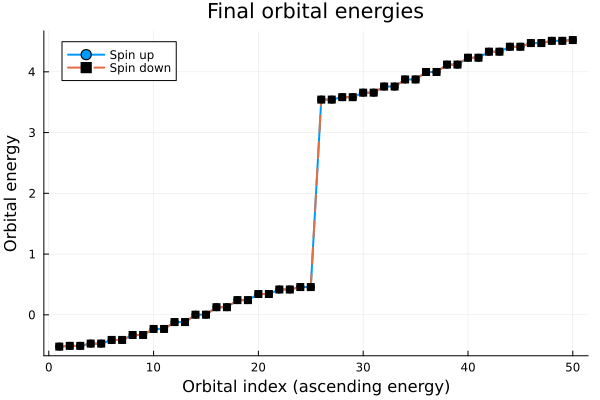
\includegraphics[width=\linewidth]{../../results_vault/experiment_04/dN00/PBC/final_orbital_energies.png}

\end{minipage}

\caption{dN00。軌道エネルギーの比較。左：OBC、右：PBC。}\end{figure}

\begin{figure}[H]\centering

\begin{minipage}{0.49\linewidth}\centering

\textbf{OBC：収束}\par

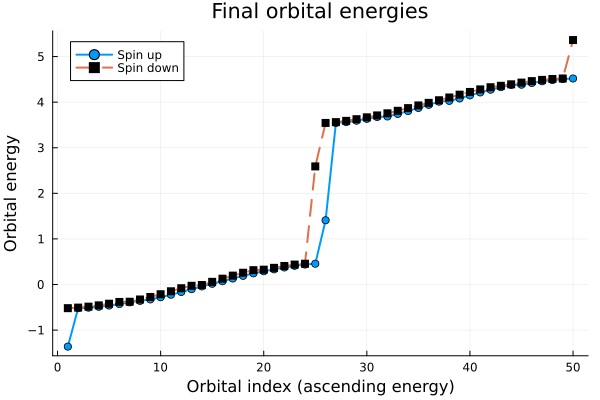
\includegraphics[width=\linewidth]{../../results_vault/experiment_04/dN02/OBC/final_orbital_energies.png}

\end{minipage}\hfill%
\begin{minipage}{0.49\linewidth}\centering

\textbf{PBC：未収束・暫定}\par

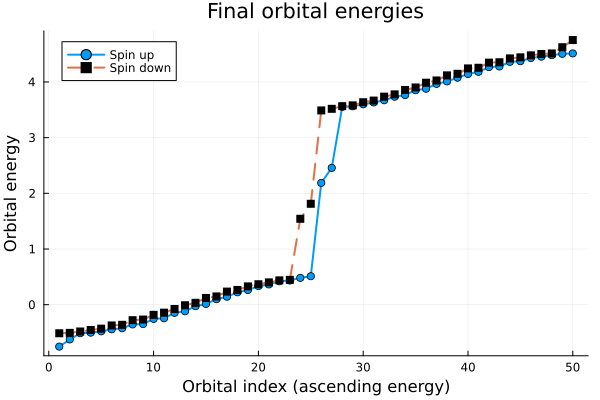
\includegraphics[width=\linewidth]{../../results_vault/experiment_04/dN02/PBC/final_orbital_energies.png}

\end{minipage}

\caption{dN02。軌道エネルギーの比較。左：OBC、右：PBC。}\end{figure}

\begin{figure}[H]\centering

\begin{minipage}{0.49\linewidth}\centering

\textbf{OBC：収束}\par

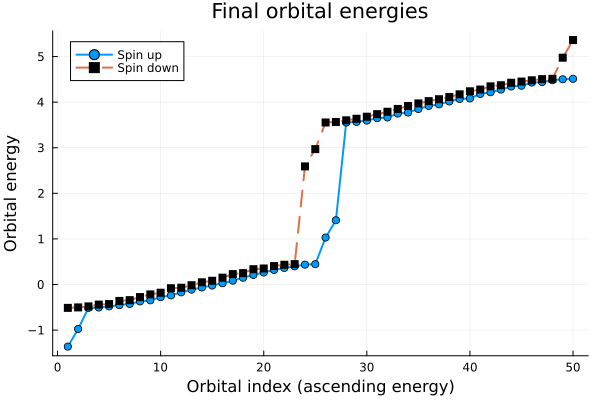
\includegraphics[width=\linewidth]{../../results_vault/experiment_04/dN04/OBC/final_orbital_energies.png}

\end{minipage}\hfill%
\begin{minipage}{0.49\linewidth}\centering

\textbf{PBC：収束}\par

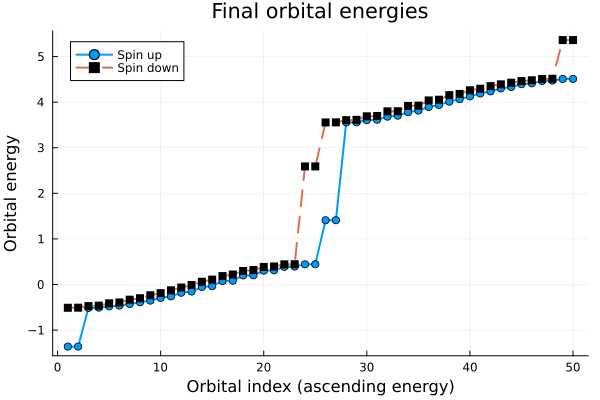
\includegraphics[width=\linewidth]{../../results_vault/experiment_04/dN04/PBC/final_orbital_energies.png}

\end{minipage}

\caption{dN04。軌道エネルギーの比較。左：OBC、右：PBC。}\end{figure}

\begin{figure}[H]\centering

\begin{minipage}{0.49\linewidth}\centering

\textbf{OBC：収束}\par

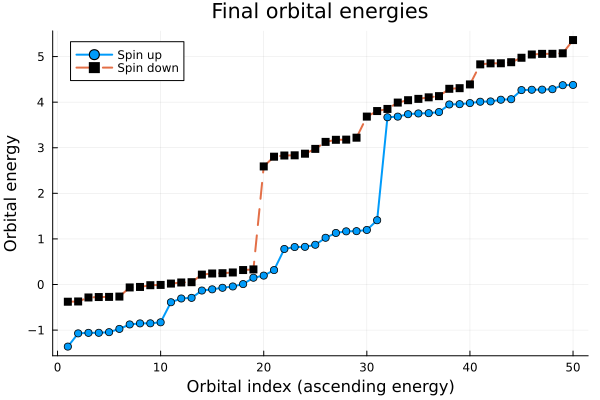
\includegraphics[width=\linewidth]{../../results_vault/experiment_04/dN12/OBC/final_orbital_energies.png}

\end{minipage}\hfill%
\begin{minipage}{0.49\linewidth}\centering

\textbf{PBC：収束}\par

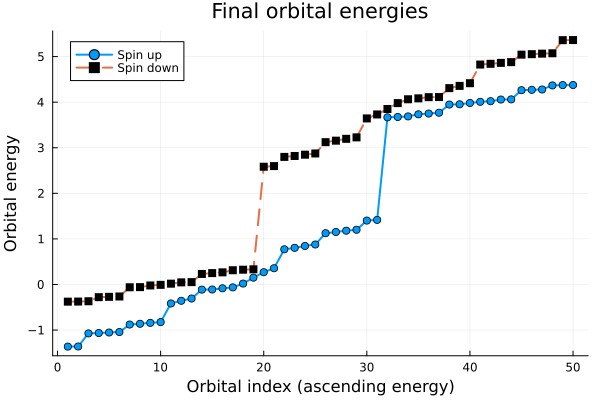
\includegraphics[width=\linewidth]{../../results_vault/experiment_04/dN12/PBC/final_orbital_energies.png}

\end{minipage}

\caption{dN12。軌道エネルギーの比較。左：OBC、右：PBC。}\end{figure}

\chapter{局所磁化：空間構造}

\sourcefile{final_magnetization.png}

OBCの $\overline{|m|}$ は0.773051から0.794301へ増える一方、$M_{\rm AF}$ は0.773051から0.273400へ下がる。図では正の磁化が連続する箇所など、単純な交互配列から外れる領域が現れる。これは全サイトが一様に強磁性化したことを意味しない。境界条件によって変調の位置も異なり、同じ平均磁化でも局所構造は一致しない。

$\overline{|m|}=L^{-1}\sum_i|m_i|$、$M_{\rm AF}=|L^{-1}\sum_i(-1)^im_i|$ と定義する。$m_i$ はスピン密度差であり、$\langle S_i^z\rangle=m_i/2$ に対応する。全磁化は $\sum_i m_i=\Delta N$ と粒子数制約で固定される。

\begin{center}\small\setlength{\tabcolsep}{4pt}
\begin{longtable}{lrrr}
\toprule
条件/境界 & 状態 & $\overline{|m|}$ & $M_{\rm AF}$ \\ \midrule
\endhead
dN00/OBC & 収束 & 0.773051 & 0.773051 \\
dN00/PBC & 収束 & 0.768964 & 0.768964 \\
dN02/OBC & 収束 & 0.778732 & 0.739615 \\
dN02/PBC & 未 & 0.739132 & 0.718574 \\
dN04/OBC & 収束 & 0.780499 & 0.643143 \\
dN04/PBC & 収束 & 0.780327 & 0.702093 \\
dN12/OBC & 収束 & 0.794301 & 0.273400 \\
dN12/PBC & 収束 & 0.794122 & 0.332345 \\
\bottomrule\end{longtable}\end{center}

\begin{figure}[H]\centering

\begin{minipage}{0.49\linewidth}\centering

\textbf{OBC：収束}\par

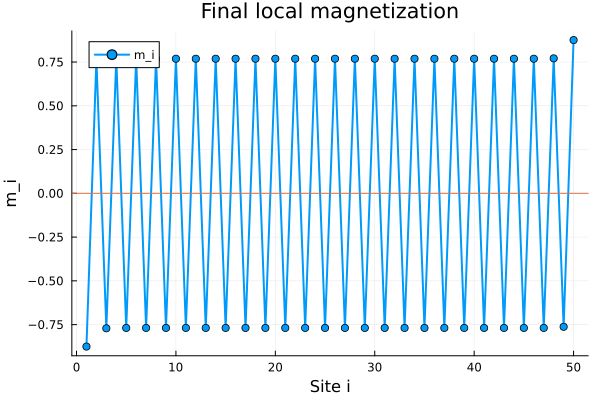
\includegraphics[width=\linewidth]{../../results_vault/experiment_04/dN00/OBC/final_magnetization.png}

\end{minipage}\hfill%
\begin{minipage}{0.49\linewidth}\centering

\textbf{PBC：収束}\par

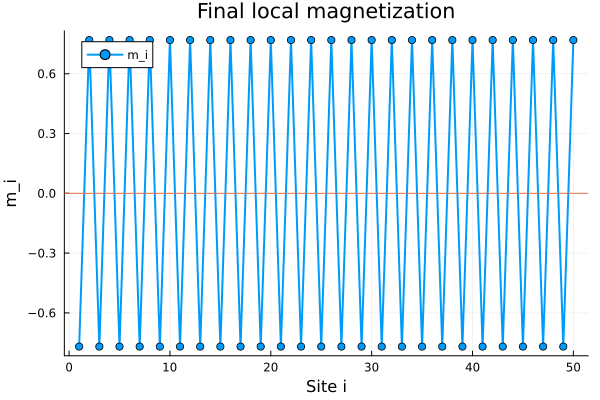
\includegraphics[width=\linewidth]{../../results_vault/experiment_04/dN00/PBC/final_magnetization.png}

\end{minipage}

\caption{dN00。局所磁化の比較。左：OBC、右：PBC。}\end{figure}

\begin{figure}[H]\centering

\begin{minipage}{0.49\linewidth}\centering

\textbf{OBC：収束}\par

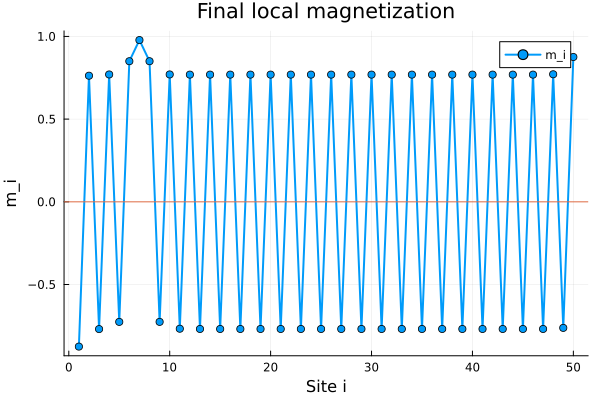
\includegraphics[width=\linewidth]{../../results_vault/experiment_04/dN02/OBC/final_magnetization.png}

\end{minipage}\hfill%
\begin{minipage}{0.49\linewidth}\centering

\textbf{PBC：未収束・暫定}\par

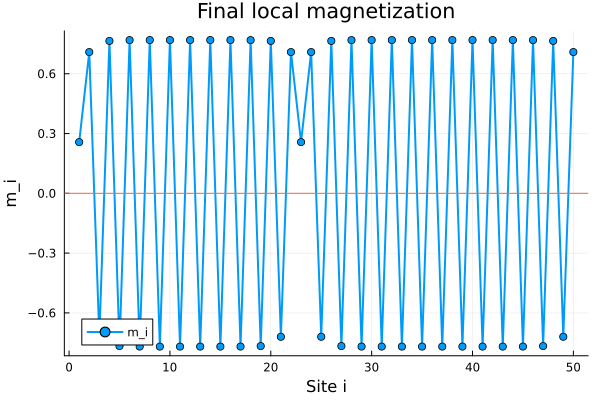
\includegraphics[width=\linewidth]{../../results_vault/experiment_04/dN02/PBC/final_magnetization.png}

\end{minipage}

\caption{dN02。局所磁化の比較。左：OBC、右：PBC。}\end{figure}

\begin{figure}[H]\centering

\begin{minipage}{0.49\linewidth}\centering

\textbf{OBC：収束}\par

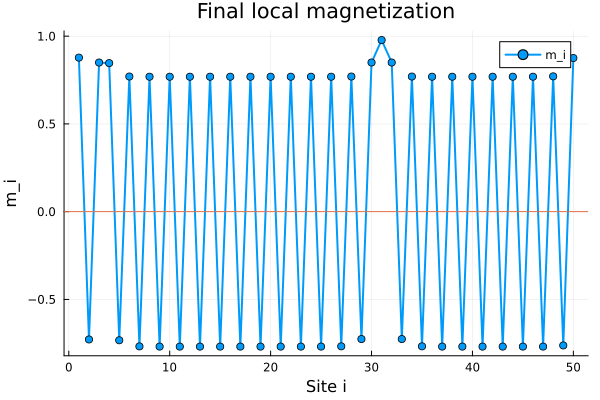
\includegraphics[width=\linewidth]{../../results_vault/experiment_04/dN04/OBC/final_magnetization.png}

\end{minipage}\hfill%
\begin{minipage}{0.49\linewidth}\centering

\textbf{PBC：収束}\par

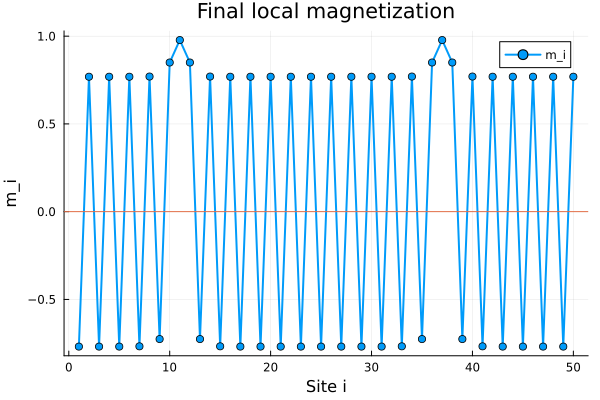
\includegraphics[width=\linewidth]{../../results_vault/experiment_04/dN04/PBC/final_magnetization.png}

\end{minipage}

\caption{dN04。局所磁化の比較。左：OBC、右：PBC。}\end{figure}

\begin{figure}[H]\centering

\begin{minipage}{0.49\linewidth}\centering

\textbf{OBC：収束}\par

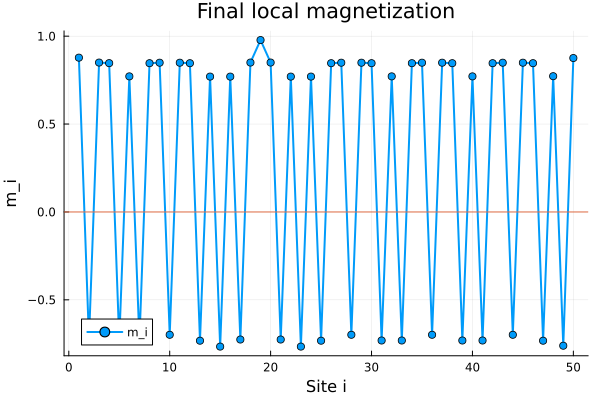
\includegraphics[width=\linewidth]{../../results_vault/experiment_04/dN12/OBC/final_magnetization.png}

\end{minipage}\hfill%
\begin{minipage}{0.49\linewidth}\centering

\textbf{PBC：収束}\par

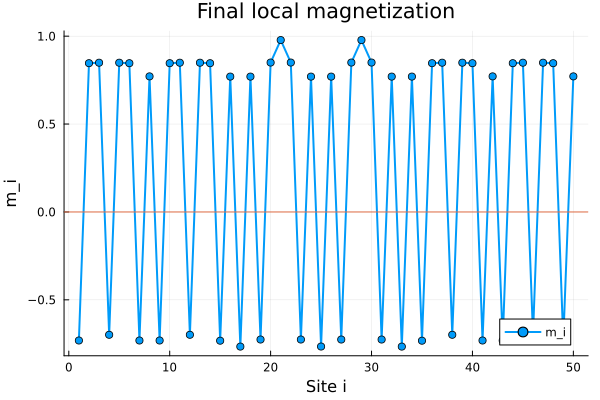
\includegraphics[width=\linewidth]{../../results_vault/experiment_04/dN12/PBC/final_magnetization.png}

\end{minipage}

\caption{dN12。局所磁化の比較。左：OBC、右：PBC。}\end{figure}

\chapter{境界条件による全エネルギー差}

\sourcefile{boundary_energy_difference.png}

$\Delta E_{\rm boundary}=E_{\rm PBC}-E_{\rm OBC}$ と定義する。負ならPBC、正ならOBCの保存された解の方が低エネルギーである。両方が収束した組だけを表と図で数値比較し、それ以外をNCとする。

$\Delta N=0$ の差は負だが、4では $+0.016109441914$、12では $+0.016059080237$ となり、得られた収束解ではOBCの方がわずかに低い。PBCが常に低エネルギーとは限らない。ただし初期条件探索による大域的最小値の保証はなく、これは今回到達した自己無撞着解同士の比較である。2の差は未収束のため判断できない。

\begin{center}\small\setlength{\tabcolsep}{4pt}
\begin{longtable}{lrr}
\toprule
条件 & $\Delta E_{\rm boundary}$ & $\Delta E_{\rm boundary}/L$ \\ \midrule
\endhead
dN00 & -0.442191290827 & -0.008843825817 \\
dN02 & NC & NC \\
dN04 & 0.016109441914 & 0.000322188838 \\
dN12 & 0.016059080237 & 0.000321181605 \\
\bottomrule\end{longtable}\end{center}

\begin{figure}[H]\centering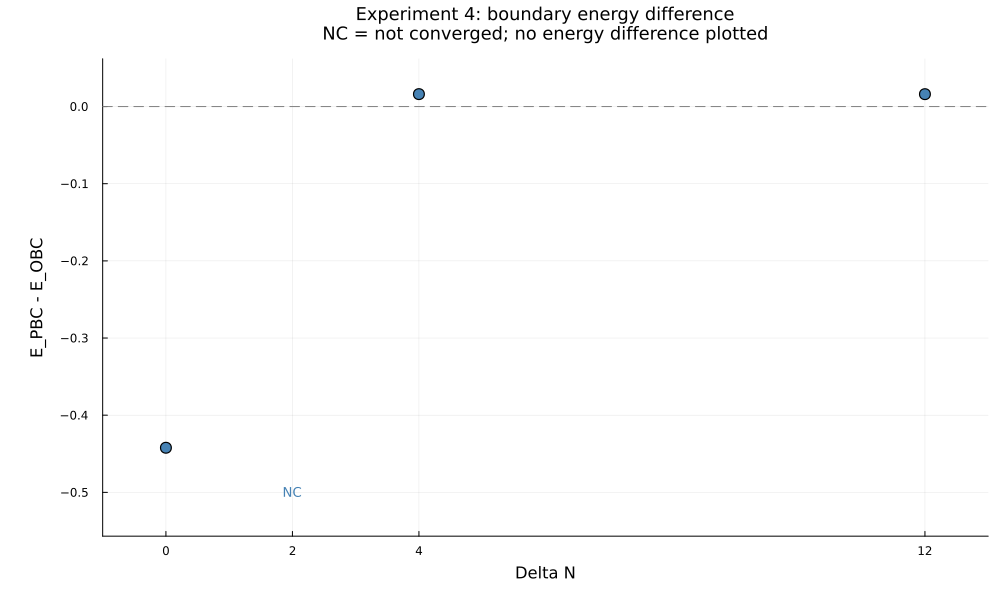
\includegraphics[width=0.9\linewidth]{../../results_vault/experiment_04/boundary_energy_difference.png}\caption{保存済みの境界エネルギー差。NCは未収束の組を示し、差が0であることを意味しない。}\end{figure}

\section*{結論と残された確認}

半充填を保って $\Delta N=0,2,4,12$ と増やす。OBCは全条件で収束し、PBCは $\Delta N=2$ のみ未収束となった。OBCのエネルギーは偏極とともに上昇するが、局所磁化の平均絶対値はわずかに増大する。磁化の振幅と交互配列の整合性は別の量である。

未収束ケースについては残差を満たす解を得た上で、複数の初期密度から同じ状態に到達するかを確認する必要がある。

サイズは50に固定しているため、境界効果と有限サイズ効果の切り分けには別サイズの結果が必要である。

\end{document}